
\section{Das RST-System}
\label{section:rst}
\begin{frame}%STARTCONTENT

\frametitle{Das RST-System}
Qualität der Funkverbindung hängt ab von

\begin{itemize}
  \item Sendeleistung
  \item verwendete Antenne
  \item Entfernung
  \item aktuelle Ausbreitungsbedingungen
  \end{itemize}
    \pause
    Im Rapport beschreibt die empfangende Station die Qualität der Verbindung

\end{frame}

\begin{frame}
\only<1>{
\begin{QQuestion}{BE201}{Was versteht man unter dem RST-Rapport? Es ist eine Kurzformel,~...}{um die Sendeleistung zu beschreiben.}
{um die Empfangsqualität zu beschreiben.}
{um den Ionosphärenzustand zu beschreiben.}
{um die Sonnenfleckenaktivität zu beschreiben.}
\end{QQuestion}

}
\only<2>{
\begin{QQuestion}{BE201}{Was versteht man unter dem RST-Rapport? Es ist eine Kurzformel,~...}{um die Sendeleistung zu beschreiben.}
{\textbf{\textcolor{DARCgreen}{um die Empfangsqualität zu beschreiben.}}}
{um den Ionosphärenzustand zu beschreiben.}
{um die Sonnenfleckenaktivität zu beschreiben.}
\end{QQuestion}

}
\end{frame}

\begin{frame}
\frametitle{RST-System}
\begin{table}
\begin{DARCtabular}{llll}
     Wert  & Bereich  & Bedeutung  & Englisch   \\
     R  & 1 -- 5  & Lesbarkeit  & Readability   \\
     S  & 1 -- 9  & Signalstärke  & Signal Strength   \\
     T  & 1 -- 9  & Tonqualität  & Tone   \\
\end{DARCtabular}
\caption{Die Bestandteile des RST-Rapports}
\label{n_rst}
\end{table}

\end{frame}

\begin{frame}
\frametitle{Readability}
Subjektive Bewertung des Lesbarkeit (Verständlichkeit)

\begin{table}
\begin{DARCtabular}{ll}
     R  & Beurteilung   \\
     1  & nicht lesbar   \\
     2  & zeitweise lesbar   \\
     3 & mit Schwierigkeiten lesbar   \\
     4  & ohne Schwierigkeiten lesbar   \\
     5  & einwandfrei lesbar   \\
\end{DARCtabular}
\caption{Anhaltspunkte für die subjektive Bewertung der Lesbarkeit (Verständlichkeit)}
\label{n_rst_r}
\end{table}
\end{frame}

\begin{frame}
\frametitle{Signal Strength}
Vom Funkgerät ablesen


\begin{figure}
    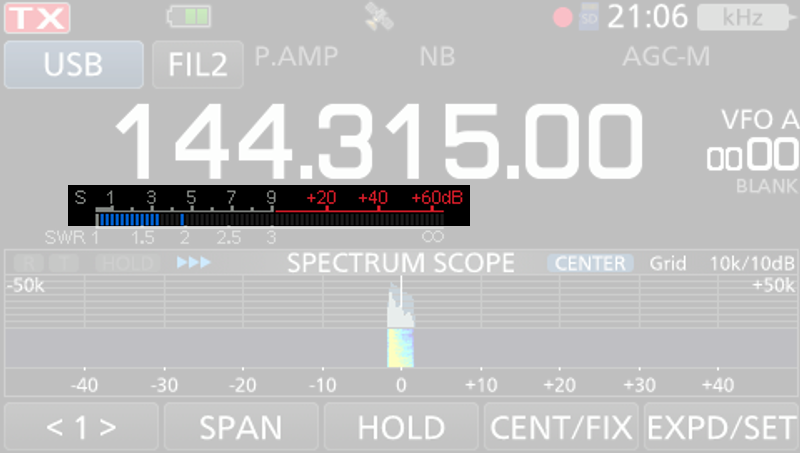
\includegraphics[width=0.85\textwidth]{foto/123}
    \caption{\scriptsize Display eines IC9700-Transceivers, hervorgehoben ist das S-Meter, das den aktuellen Empfangspegel anzeigt}
    \label{n_rst_s-meter}
\end{figure}

\end{frame}

\begin{frame}
\frametitle{Beispiele für RST-Rapporte}
im Sprechfunk

\begin{table}
\begin{DARCtabular}{llcl}
     Verständlichkeit  & S-Meter  &$\rightarrow$ & RST-Rapport   \\
     einwandfrei (=5)  & +\qty{20}{\dB}  &$\rightarrow$ & 59+20dB   \\
     einwandfrei (=5)  & 9  &$\rightarrow$ & 59   \\
     ohne Schwierigkeiten (=4)  & 5  &$\rightarrow$ & 45   \\
     mit Schwierigkeiten (=3)  & 3  &$\rightarrow$ & 33   \\
     unverständlich (=1)  & 3  &$\rightarrow$ & 13   \\
\end{DARCtabular}
\caption{Beispiele für RST-Rapporte im Sprechfunk}
\label{n_rst_beispiele}
\end{table}
\end{frame}

\begin{frame}
\only<1>{
\begin{QQuestion}{BE202}{Was bedeuten die Buchstaben RST, mit denen Sie die Empfangsqualität einer Sendung beurteilen können?}{R = Rufzeichen, S = Standort, T = Tonqualität}
{R = Rufzeichen, S = Signalstärke, T = Tonqualität}
{R = Lesbarkeit, S = Signalstärke, T = Trägerfrequenz}
{R = Lesbarkeit, S = Signalstärke, T = Tonqualität}
\end{QQuestion}

}
\only<2>{
\begin{QQuestion}{BE202}{Was bedeuten die Buchstaben RST, mit denen Sie die Empfangsqualität einer Sendung beurteilen können?}{R = Rufzeichen, S = Standort, T = Tonqualität}
{R = Rufzeichen, S = Signalstärke, T = Tonqualität}
{R = Lesbarkeit, S = Signalstärke, T = Trägerfrequenz}
{\textbf{\textcolor{DARCgreen}{R = Lesbarkeit, S = Signalstärke, T = Tonqualität}}}
\end{QQuestion}

}
\end{frame}

\begin{frame}
\only<1>{
\begin{QQuestion}{BE203}{In welcher Weise wird nach dem RST-System die Empfangsqualität einer Amateurfunkaussendung beurteilt?}{Lesbarkeit in Stufen von 1-5,  Signalstärke in Stufen von 1-5 und  Tonhöhe in Stufen von 1-9}
{Lesbarkeit in Stufen von 1-5,  Signalstärke in Stufen von 1-9 und  Tonqualität in Stufen von 1-9}
{Signalqualität in Stufen von 1-5,  Signalstärke in Stufen von 1-5 und  Tonqualität in Stufen von 1-9}
{Lesbarkeit in Stufen von 1-9,  Signalqualität in Stufen von 1-5 und  Tonhöhe in Stufen von 1-4}
\end{QQuestion}

}
\only<2>{
\begin{QQuestion}{BE203}{In welcher Weise wird nach dem RST-System die Empfangsqualität einer Amateurfunkaussendung beurteilt?}{Lesbarkeit in Stufen von 1-5,  Signalstärke in Stufen von 1-5 und  Tonhöhe in Stufen von 1-9}
{\textbf{\textcolor{DARCgreen}{Lesbarkeit in Stufen von 1-5,  Signalstärke in Stufen von 1-9 und  Tonqualität in Stufen von 1-9}}}
{Signalqualität in Stufen von 1-5,  Signalstärke in Stufen von 1-5 und  Tonqualität in Stufen von 1-9}
{Lesbarkeit in Stufen von 1-9,  Signalqualität in Stufen von 1-5 und  Tonhöhe in Stufen von 1-4}
\end{QQuestion}

}
\end{frame}

\begin{frame}
\only<1>{
\begin{PQuestion}{NF103}{Die Darstellung zeigt das Display eines Transceivers im Empfangsbetrieb. Wie wird die Anzeige 2 bezeichnet?}{Amplitudenspektrum}
{S-Meter}
{SWR-Meter}
{Wasserfalldiagramm}
{\DARCimage{1.0\linewidth}{579include}}\end{PQuestion}

}
\only<2>{
\begin{PQuestion}{NF103}{Die Darstellung zeigt das Display eines Transceivers im Empfangsbetrieb. Wie wird die Anzeige 2 bezeichnet?}{Amplitudenspektrum}
{\textbf{\textcolor{DARCgreen}{S-Meter}}}
{SWR-Meter}
{Wasserfalldiagramm}
{\DARCimage{1.0\linewidth}{579include}}\end{PQuestion}

}
\end{frame}

\begin{frame}
\only<1>{
\begin{QQuestion}{NF301}{Zu welchem Zweck dient das S-Meter in einem Transceiver?}{Es dient zur Anzeige der Sendeleistung.}
{Es dient zur Anzeige des Empfangspegels.}
{Es dient zur Anzeige der Empfängerverstärkung.}
{Es dient zur Anzeige der Audiolautstärke.}
\end{QQuestion}

}
\only<2>{
\begin{QQuestion}{NF301}{Zu welchem Zweck dient das S-Meter in einem Transceiver?}{Es dient zur Anzeige der Sendeleistung.}
{\textbf{\textcolor{DARCgreen}{Es dient zur Anzeige des Empfangspegels.}}}
{Es dient zur Anzeige der Empfängerverstärkung.}
{Es dient zur Anzeige der Audiolautstärke.}
\end{QQuestion}

}
\end{frame}

\begin{frame}Bei den folgenden Prüfungsfragen kommt es darauf an das S-Meter richtig abzulesen. In allen Prüfungsfragen wird von einem einwandfreien Signal in Telefonie (Sprechfunk) ausgegangen. Der R-Wert ist daher jeweils 5 und der T-Wert entfällt.

\end{frame}

\begin{frame}
\only<1>{
\begin{PQuestion}{BE204}{Sie hören die Gegenstation in SSB-Telefonie einwandfrei. Das Anzeigeinstrument Ihres Funkgerätes zeigt den dargestellten Zeigerausschlag. Welchen Rapport nach dem RST-System geben Sie?}{25}
{29}
{52}
{55}
{\DARCimage{1.0\linewidth}{421include}}\end{PQuestion}

}
\only<2>{
\begin{PQuestion}{BE204}{Sie hören die Gegenstation in SSB-Telefonie einwandfrei. Das Anzeigeinstrument Ihres Funkgerätes zeigt den dargestellten Zeigerausschlag. Welchen Rapport nach dem RST-System geben Sie?}{25}
{29}
{52}
{\textbf{\textcolor{DARCgreen}{55}}}
{\DARCimage{1.0\linewidth}{421include}}\end{PQuestion}

}
\end{frame}

\begin{frame}
\only<1>{
\begin{PQuestion}{BE205}{Sie hören die Gegenstation in SSB-Telefonie einwandfrei. Das Anzeigeinstrument Ihres Funkgerätes zeigt den dargestellten Zeigerausschlag. Welchen Rapport nach dem RST-System geben Sie?}{95}
{39}
{59}
{56}
{\DARCimage{1.0\linewidth}{420include}}\end{PQuestion}

}
\only<2>{
\begin{PQuestion}{BE205}{Sie hören die Gegenstation in SSB-Telefonie einwandfrei. Das Anzeigeinstrument Ihres Funkgerätes zeigt den dargestellten Zeigerausschlag. Welchen Rapport nach dem RST-System geben Sie?}{95}
{39}
{\textbf{\textcolor{DARCgreen}{59}}}
{56}
{\DARCimage{1.0\linewidth}{420include}}\end{PQuestion}

}
\end{frame}

\begin{frame}
\only<1>{
\begin{PQuestion}{BE206}{Sie hören die Gegenstation in SSB-Telefonie einwandfrei. Das Anzeigeinstrument Ihres Funkgerätes zeigt den dargestellten Zeigerausschlag. Welchen Rapport nach dem RST-System geben Sie?}{520}
{69}
{4,2}
{59+\qty{20}{\decibel}}
{\DARCimage{1.0\linewidth}{422include}}\end{PQuestion}

}
\only<2>{
\begin{PQuestion}{BE206}{Sie hören die Gegenstation in SSB-Telefonie einwandfrei. Das Anzeigeinstrument Ihres Funkgerätes zeigt den dargestellten Zeigerausschlag. Welchen Rapport nach dem RST-System geben Sie?}{520}
{69}
{4,2}
{\textbf{\textcolor{DARCgreen}{59+\qty{20}{\decibel}}}}
{\DARCimage{1.0\linewidth}{422include}}\end{PQuestion}

}
\end{frame}

\begin{frame}
\only<1>{
\begin{PQuestion}{BE207}{Sie hören in einem Funkgespräch in SSB-Telefonie die Gegenstation einwandfrei. Das Display Ihres Funkgerätes zeigt die abgebildeten Informationen an. Welchen Empfangsrapport nach dem RST-System geben Sie?}{100}
{7}
{55}
{1}
{\DARCimage{1.0\linewidth}{587include}}\end{PQuestion}

}
\only<2>{
\begin{PQuestion}{BE207}{Sie hören in einem Funkgespräch in SSB-Telefonie die Gegenstation einwandfrei. Das Display Ihres Funkgerätes zeigt die abgebildeten Informationen an. Welchen Empfangsrapport nach dem RST-System geben Sie?}{100}
{7}
{\textbf{\textcolor{DARCgreen}{55}}}
{1}
{\DARCimage{1.0\linewidth}{587include}}\end{PQuestion}

}
\end{frame}

\begin{frame}
\only<1>{
\begin{PQuestion}{BE208}{Sie hören in einem Funkgespräch in SSB-Telefonie die Gegenstation einwandfrei. Das Display Ihres Funkgerätes zeigt die abgebildeten Informationen an. Welchen Empfangsrapport nach dem RST-System geben Sie?}{80}
{12,5}
{59}
{95}
{\DARCimage{1.0\linewidth}{586include}}\end{PQuestion}

}
\only<2>{
\begin{PQuestion}{BE208}{Sie hören in einem Funkgespräch in SSB-Telefonie die Gegenstation einwandfrei. Das Display Ihres Funkgerätes zeigt die abgebildeten Informationen an. Welchen Empfangsrapport nach dem RST-System geben Sie?}{80}
{12,5}
{\textbf{\textcolor{DARCgreen}{59}}}
{95}
{\DARCimage{1.0\linewidth}{586include}}\end{PQuestion}

}
\end{frame}

\begin{frame}
\only<1>{
\begin{PQuestion}{BE209}{Sie hören in einem Funkgespräch in SSB-Telefonie die Gegenstation einwandfrei. Das Display Ihres Funkgerätes zeigt die abgebildeten Informationen an. Welchen Empfangsrapport nach dem RST-System geben Sie?}{59+\qty{20}{\decibel}}
{520}
{50}
{17}
{\DARCimage{1.0\linewidth}{588include}}\end{PQuestion}

}
\only<2>{
\begin{PQuestion}{BE209}{Sie hören in einem Funkgespräch in SSB-Telefonie die Gegenstation einwandfrei. Das Display Ihres Funkgerätes zeigt die abgebildeten Informationen an. Welchen Empfangsrapport nach dem RST-System geben Sie?}{\textbf{\textcolor{DARCgreen}{59+\qty{20}{\decibel}}}}
{520}
{50}
{17}
{\DARCimage{1.0\linewidth}{588include}}\end{PQuestion}

}
\end{frame}%ENDCONTENT
